\documentclass[a4paper,10pt,twoside]{cpc-hepnp}

\usepackage{multicol}
\usepackage{graphicx}
\usepackage{booktabs}
\usepackage{amssymb,bm,mathrsfs,bbm,amscd}
\usepackage[tbtags]{amsmath}
\usepackage{lastpage}
\usepackage{lineno}
\usepackage{ifpdf}
\usepackage{subfigure}
\ifpdf
   \DeclareGraphicsRule{*}{mps}{*}{}
\else
   \DeclareGraphicsRule{*}{eps}{*}{}
\fi

\linenumbers

\renewcommand{\mathstrut}{\protect\vphantom{\hat{0123456789}}}

%\linespread{2} % comment this after all the revision
\begin{document}



\fancyhead[c]{\small Chinese Physics C~~~Vol. xx, No. x (2017) xxxxxx}
\fancyfoot[C]{\small 010201-\thepage}

%\footnotetext[0]{Received 14 March 2009}


\title{Fast simulation of the CEPC detector with {\textsc{Delphes}} and its validation
\thanks{The study was partially supported by the CAS/SAFEA International Partnership Program for Creative Research Teams?and funding from CAS and IHEP for the Thousand Talent and Hundred Talent programs, as well as grants from the State Key Laboratory of Nuclear Electronics and Particle Detectors.}}

\author{%
      Xin. Mo$^{1)}$%
\quad Cheng Chen$^{2}$
\quad Gang Li$^{1)}$\email{li.gang@ihep.ac.cn}%
\quad Manqi Ruan$^{1)}$\email{manqi.ruan@ihep.ac.cn}%
\quad Qiang Li$^{2}$
\quad Xinchou Lou$^{1,3)}$%
}
\maketitle


\address{%
$^1$ Institute of High Energy Physics, Chinese Academy of Sciences, Beijing 100049, China\\
$^2$ Peking University, Beijing, China\\ 
$^3$ University of Texas at Dallas, Richardson, TX 75080-3021, USA
}


\begin{abstract}
In this paper, the {\textsc{Delphes}~} is used to simulate the detector at the Circular Electron-Positron Collider (CEPC).
The geometry and performance of the CEPC detector are presented and validated with a series of benchmark processes.
The comparisons between {\textsc{Delphes}~} and the full simulation, which is based on Geant4 \& Marlin,
show that {\textsc{Dephes}} simulates the CEPC detector well.
The differences of physics analysis between hadron and lepton collider are also stressed.  
\end{abstract}


\begin{keyword}
CEPC, {\textsc{Delphes}~}, fast simulation
\end{keyword}

\begin{pacs}
%1---3 PACS(Physics and Astronomy Classification Scheme, http://www.aip.org/pacs/pacs.html/)
13.66.Fg, 14.80.Bn, 07.05.-t
\end{pacs}

\footnotetext[0]{\hspace*{-3mm}\raisebox{0.3ex}{$\scriptstyle\copyright$}2013
Chinese Physical Society and the Institute of High Energy Physics
of the Chinese Academy of Sciences and the Institute
of Modern Physics of the Chinese Academy of Sciences and IOP Publishing Ltd}%

\begin{multicols}{2}


\section{Introduction}\label{sec:intro}

CEPC\cite{ref:cepc_det, ref:cepc_acc} is a next generation electron-positron collider proposed by Chinese scientists.
The machine is expected to collide electron and positron beams at the center-of-mass energy of 240 - 250 GeV
to maximize the Higgs production cross section of the $e^+e^- \to ZH$ process, with an instantaneous luminosity of $2\times10^{34}$ cm$^{-2} s^{-1}$.
CEPC is designed to deliver a total of 5 ab$^{-1}$ integrated luminosity with two detectors in 10 years,
which means that over $10^6$ Higgs events will be produced.
The large statistics with clean backgrounds can enable CEPC to perform Higgs precision measurements,
Standard Model (SM) tests, and searches for potential new physical phenomena.
Theorists would get involved to test various new models to investigate the precisions and sensitivities of the CEPC.
In order to save computing time and to simplify the procedure of full detector simulation and reconstruction,
a dedicated fast simulation tool is highly demanded.

{\textsc{Delphes}~}\cite{ref:delphes} is a fast simulation framework developed in 2009, and the latest prime version was released in 2013,
which is widely used for phenomenological studies on the simulation of various detector designs.
The {\textsc{Delphes}~} framework simulates the response of a general purpose collider detector,
whose components are organized concentrically with a cylindrical symmetry around the beam axis.
The energy and momentum are simulated according to the detector resolutions and efficiencies required by users.
Eventually, all kinds of particles are reconstructed with algorithm based on PFA\cite{ref:pfa} philosophy,
then clustering into jets with FastJet~\cite{ref:fastjet} .

This paper is organized as following.  In Sect.{~\ref{sec:detector}}, the CEPC detector geometry are briefly introduced.
Then in Sect.{~\ref{sec:simulation}}, the MC generation, full simulation, and reconstruction chain are presented in detail,
the data analysis of $e^+e^-$  experiment is also discussed as well.
In Sect.{~\ref{sec:validation}}, a series of benchmark processes are chosen to the validate the fast simulation on CEPC
by comparing it with full simulation.
In Sect.{~\ref{b-tagging}}, the improvement of flavor tagging according to full simulation and its usage are introduced.
In the end the conclusion remarks are presented.

\section{The CEPC detector concept\label{sec:detector}}

The CEPC detector concept design\cite{ref:cepc_det} takes the ILC detector, ILD\cite{ref:ilc, ref:ild},
as a reference and adopts the philosophy of PFA,
which benefits from its precision tracking system and high granularity calorimetric system.

The CEPC detector consists of three main sub-detectors and a superconducting solenoid of 3.5 T.
The three sub-detectors are, from inner to outer,  a hybrid tracking system composed of several silicon based devices
and a Time Projection Chamber (TPC), a high granularity calorimetry system, and a Muon detector.

The hybrid tracking system has five parts. A vertex detector (VTX), constructed with high spatial resolution pixel sensor,
is placed very close to the interaction point (IP) and  the inner radius is only 16 mm.
The VTX provides very precision measurements of the impact parameters of tracks,
which is used for the $b-/c-$jet flavor tagging and $\tau$-tagging.
A Silicon Inner Tracker (SIT) is just outside and cooperating with the VTX for vertex reconstruction and flavor tagging.
A set of Forward Tracking Disks (FTDs) are placed in the forward region
to increase the geometric acceptance of tracking system with coverage up to $|\cos\theta| = 0.99$.
A Silicon External Tracker (SET) and End-cap Tracking Disks (ETD) are taken as the outermost layer of whole tracker system,
which provide precision position measurements of tracks entering the calorimetric system.
The TPC, with a 2.35m half-length and 1.8m outer radius, provides over 200 hits per track and 100 $\mu$m resolution in $r\phi$ plane,
which allows for excellent pattern recognition, track reconstruction efficiency, and potential $dE/dx$-based particle identification.

A calorimetric system consisting of Electromagnetic Calorimeter (ECAL) and Hadron Calorimeter (HCAL)
with very fine granularity is placed inside the solenoid.
The system plays an essential role in the Particle-Flow Algorithm (PFA),
providing excellent separation of showers from different particles and jet energy resolution of 3-4\%.

A superconducting solenoid of 3.5 T is surrounding the calorimetry system.
The return yoke is placed outside the solenoid. The CEPC muon system acts as the muon identifier,
the solenoid flux return yoke and the support structure for the whole spectrometer.
High muon detection efficiency, low hadron mis-identification rate,
modest position resolution and large coverage are the main concerns of the design.


\section{Monte Carlo samples, detector simulation, reconstruction, and analysis\label{sec:simulation}}

For the CEPC detector design and optimization,
a whole set of $e^+e^- \to ZH$ signal process and Standard Model (SM) backgrounds have been generated~\cite{ref:cepccpc}
with the generic Monte-Carlo generator {\sf Whizard 1.95}{~\cite{ref:whizard}}.
To simulate the detector response, a full simulation package, Mokka{~\cite{ref:mokka}},
based on Geant4{~\cite{ref:geant4}} and a fast simulation framework of the {\textsc{Delphes}~}{~\cite{ref:delphes}} are used.  The Particle Flow Algorithm (PFA) philosophy is utilized in the reconstruction of both the full and fast simulation.

%In order to validate the configuration of Delphes for the CEPC, some benchmark processes are chosen for the comparison. The first one is the Higgs inclusive decay process in the associated Z leptonic channel, which is critical for Higgs model independent measurement. The second one is the Higgs invisible decay mode, associated with hadronic Z decay channel. This channel may be sensitive to some new physics related to Higgs. The last one is Higgs decays into double W bosons, one is on-shell meanwhile the other is off-shell, and the associated Z decays into neutrinos. This benchmark channel can be valuable to constrain the SM parameters, such as HWW coupling.

After full simulation,  hits in different sub-detectors are digitized properly
and reconstructed with reconstruction software  Marlin{~\cite{ref:marlin}}.
A dedicated PFA, Arbor\cite{ref:arbor},  is used for particle reconstruction, and Pandora{~\cite{ref:pandora}}, an alternative one,
is taken as reference. All jets are reconstructed with LCFIPlus package\cite{ref:lcfiplus},
where a $e^+e^-~k_t$ algorithm{~\cite{ref:eekt}},  often referred to also as {\sf Durham} algorithm,  is used for jet-clustering.

The detector model implemented in the {\textsc{Delphes}} is same as the one in full simulation with necessary simplifications.
For the charged tracks simulated with {\textsc{Delphes}}, there is a common strategy to smear their momentum.
The angular resolution is assumed to be perfect, so that the smearing only applied to the transversal momentum.
In practice, the resolution of their momentum is described as a Gaussian and  $\Delta(1/p_t)=a \oplus (b p_t) $,
where $a$ and $b$ are taken same as CEPC pre-CDR.
The reconstruction efficiency is 100\% in the detector coverage since the it is greater than 99\% for $p_t>0.1$ GeV.
%Then the charged tracks are  reconstructed according to the user-defined probability, which are listed in Tab.~\ref{tab:tab1}.


For neutral objects which mainly rely on the calorimetric system, some points should be clarified.
The first, the fake rate for electrons, muons and photons is not implemented in the current version of {\textsc{Delphes}~};
The second, photon conversions into electron-positron pairs are ignored neither.
Both the true photons and electrons reaching calorimeter without a reconstructed track are considered as photon in {\textsc{Delphes}~}.
The resolutions of photon and neutral hadrons are taken from pre-CDR, which are consistent those of full simulation.

The overall reconstruction of particles implemented in {\textsc{Delphes}~} is mainly based on a perfect PFA.
For the charged tracks, the reconstruction involves both the tracker system and the calorimetric system.
Since the resolution of tracking system is better than this of calorimeter in the CEPC energy region,
it can be convenient to use the tracking information within the tracker acceptance for estimating the charged particle momenta.
The efficiencies could be parameterized as a function of the energy and pseudo-rapidity. But it should be borne in mind
that the detection efficiencies of fast simulation is higher than full simulation by about 5\% per photon
since the photon conversions is not simulated.   



In order to get same performance of jet-clustering, $e^+e^-~k_t$ algorithm is also used in fast simulation.
The exclusive mode of fast jet is used and the input particles are forced into fixed number of jets
without any $y_{ij}$ or $P_t$ requirements, which can be applied at analysis stage.

It is worthy to note that the analysis strategy at $e^+e^-$ collider is different from the one of hadron colliders,
such as the Atlas and the CMS.  The $e^+e^-$ experiments have much less backgrounds than hadron ones and almost pile-up free,
and usually almost all final states particles of a event are detected and used in analysis.
For instance, all the final physics objects will be used in the analysis of
$e^+e^- \to ZH,~\mbox{with}~Z \to\mu^+\mu^-~\mbox{and}~H \to 2\mbox{Jets} $.
As a consequence, the muon pair should be identified firstly with both Pid and kinematic constrains.
Then, the remain particles are forced into 2 jets with exclusive mode of $e^+e^-~k_t$ jet-clustering algorithm.
And any background contaminations of mis-combination can be suppressed in the final event selection with additional requirements.


\section{Validation with full simulation\label{sec:validation}}


On the CEPC, the full simulation is achieved with Geant4 and several toolkits based on the LCIO framework\cite{ref:lcio}.
Geant4\cite{ref:geant4} is a general simulation package suitable from single particle phenomena study to full scale detector simulation.
In the current study, the geometric structure and material information of the CEPC have been encoded as CEPC\_v1 configuration card,
which is essentially for simulating the detector responds with Geant4.
After the digitization, the detector responds are stored in the form of LCIO format.
A user interface of LCIO, named as Marlin, is provided to read all the data from simulation and reconstruct them as hits, tracks, and clusters.

Tracks and clusters then will be interpreted as the reconstructed particles with Arbor algorithm\cite{ref:arbor}.
The basic idea of Arbor algorithm is inspired by the fact that the shower spatial development  in the calorimeter follows the topology of a tree.
In calorimeter, if the distance of a pair of hits is less than a predefined threshold, a connector will be established for the pair.
To avoid loop connectors or multiple connectors to a single hit,
a cleaning procedure is implemented to ensure that at each hit there is at most one connector which with minimum angle
to a well selected direction.
After all tree structure of shower completed, the shower would be merged with a track if it is charged or not.


The fast simulation and its reconstruction in {\textsc{Delphes}~} must be validated by comparing the relative distributions
of all types of physics objects to those of full simulation, as well as the efficiencies.
Several benchmark processes are selected, which cover all the physics objects of CEPC experiments, such as leptons, photons, and jets.


\subsection{$e^+e^-\to \mu^+\mu^-H$}

The $e^+e^- \to \mu^+\mu^-H$ process is one of the most important analysis on at $e^+e^-$ Higgs factory,
which enables the model-independent measurement of Higgs mass and production rate.
The di-muons come from Z boson decay and Higgs is tagged from the recoiling side, since the initial four-momentum is precisely defined.
So the study on the recoil mass distribution produces important properties of the Higgs but without detecting any Higgs decay products.
Fig.~\ref{fig:mumuh} shows the comparisons of invariant mass of and recoil mass against $\mu^+\mu^-$ pair between fast and full simulations.
It can be found that these two are consistent very well.

\begin{center}
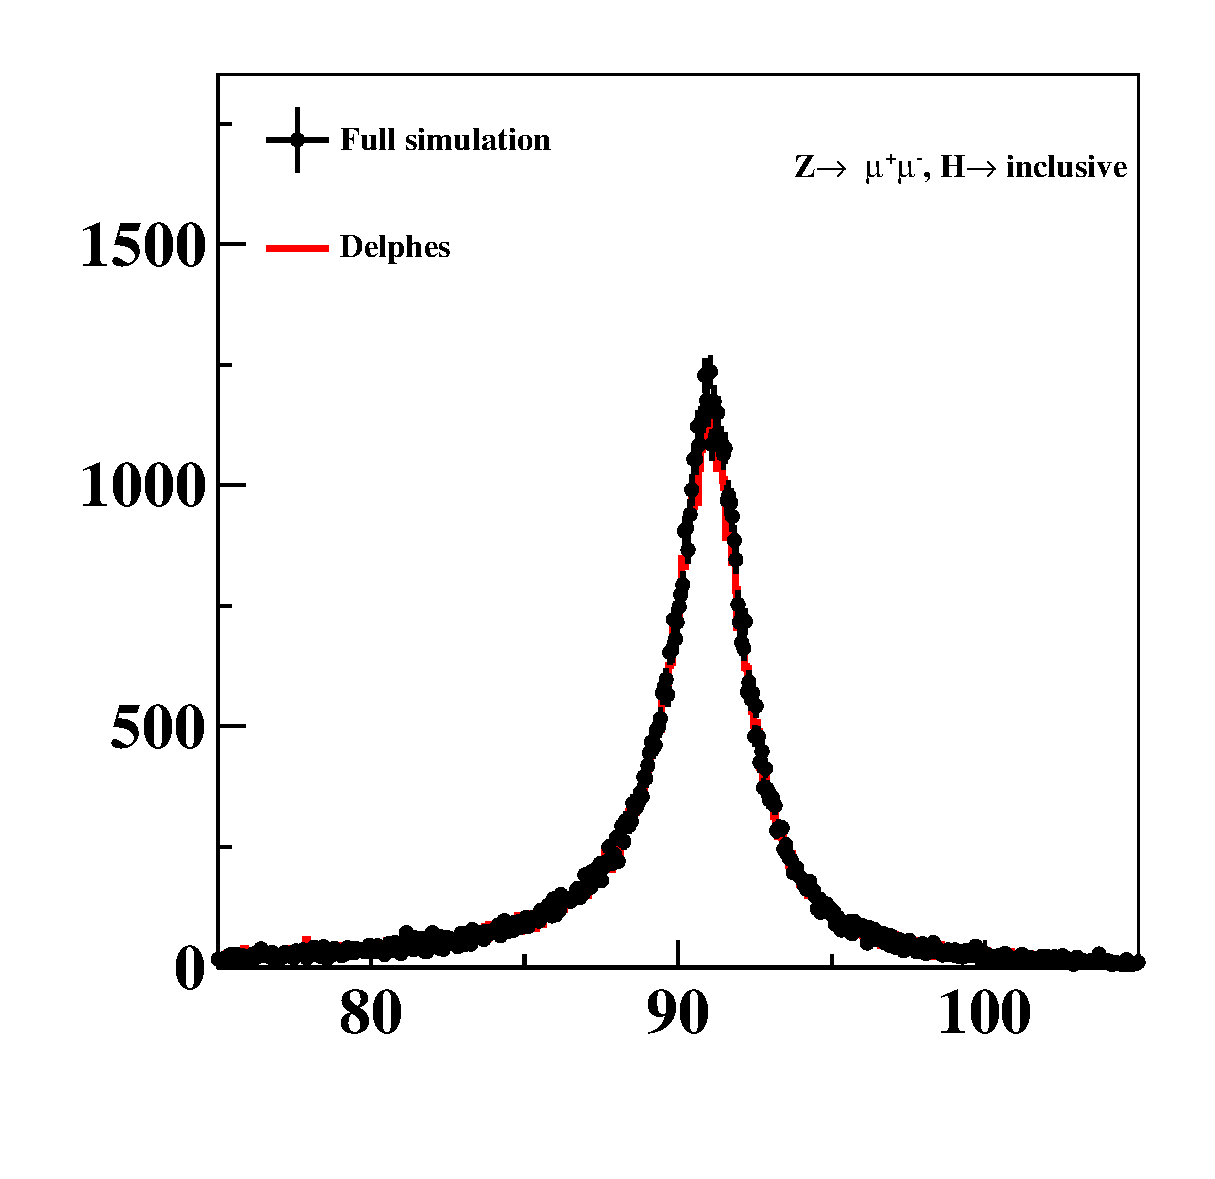
\includegraphics[width=0.45\linewidth]{figs/e2e2h_mass}
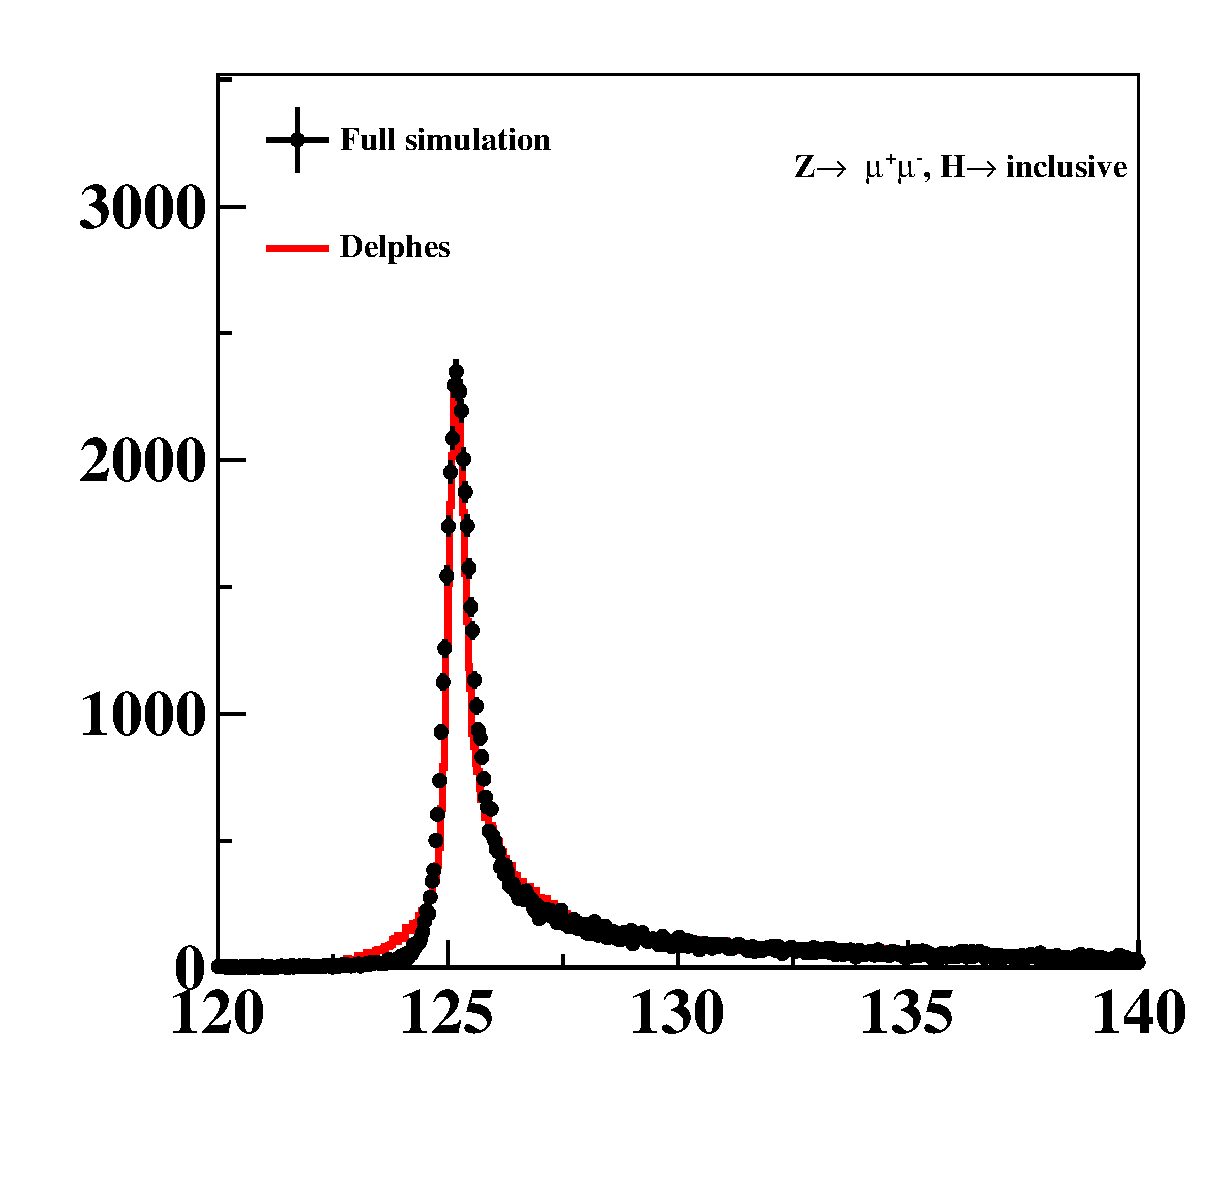
\includegraphics[width=0.45\linewidth]{figs/e2e2h_reco}
\figcaption{\label{fig:mumuh}The invariant mass (left) of and recoil mass (right) against $\mu^+\mu^-$ distributions in $e^+e^- \to ZH$,
  $Z \to \mu^+\mu^-$ and $H \to \mbox{inclusive}$. The dot with error bar and red histogram represent full and fast simulation, respectively (same in the following plots).
}
\end{center}

\subsection{$e^+e^-\to \nu\bar{\nu}H$, $H \to \gamma \gamma$}
To validate the detection of photon in the CEPC detector conceptual design,
the $e^+e^- \to \nu\bar{\nu}H$, $H\to \gamma \gamma$ is taken as an example.
There are only two isolated photon in the final state if the initial state radiation (ISR) photons are neglected.
Fig.~\ref{fig:hgg} shows the comparison between fast and full simulation,
it can seen that the energy resolution of photon is well modeled by fast simulation.
But it should be noted that the photon conversion effect is not taken into account in the fast simulation
and its photon detection efficiency is higher than full simulation.
\begin{center}
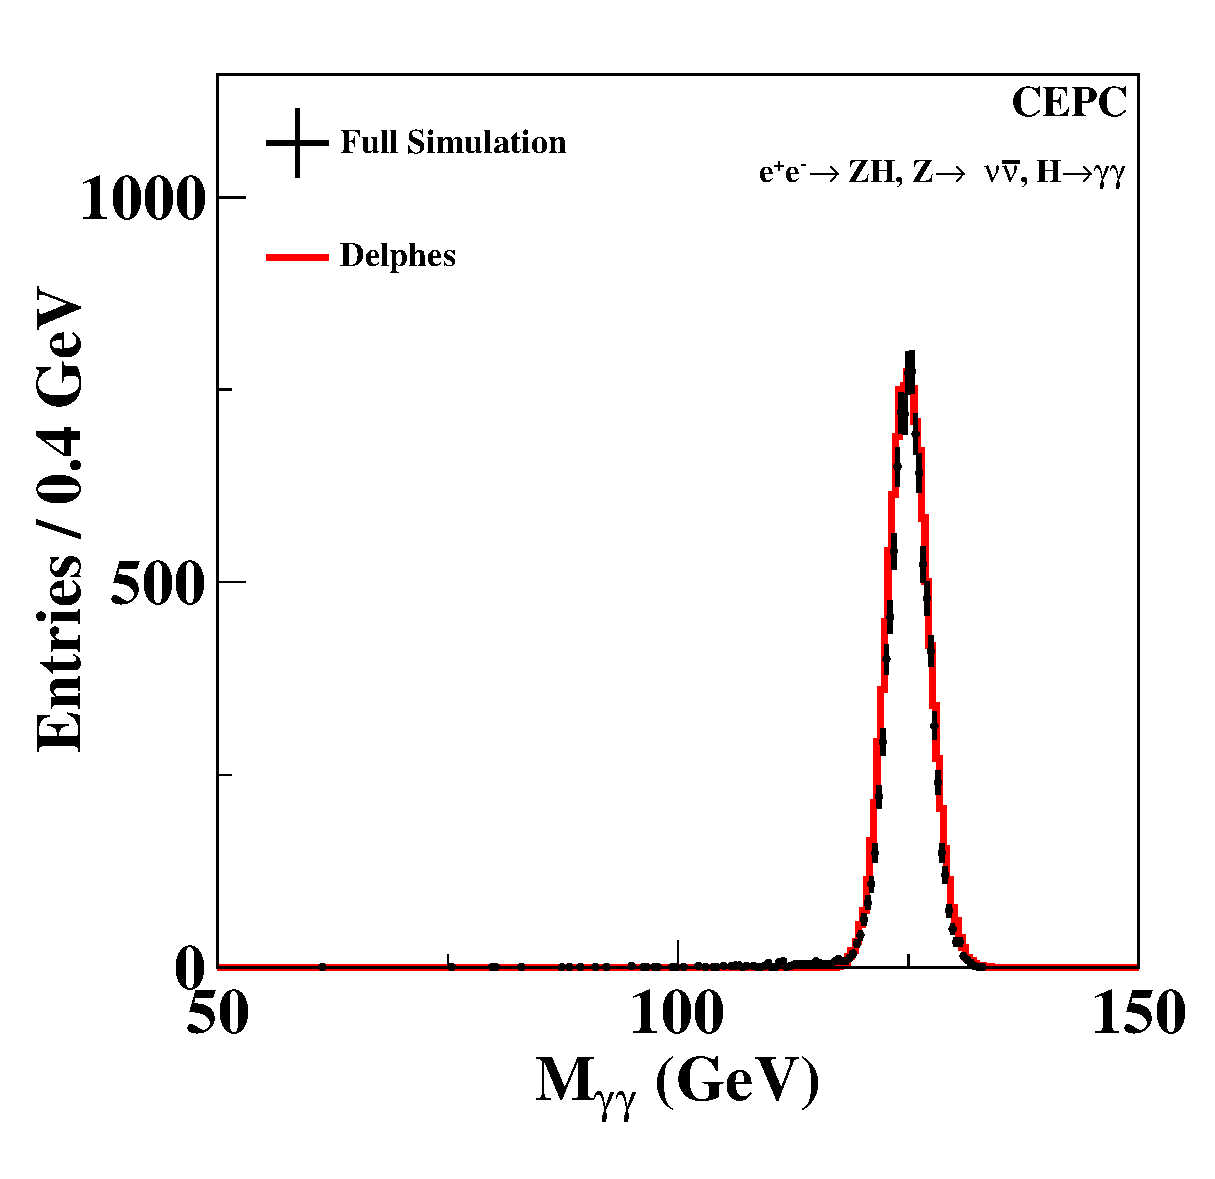
\includegraphics[width=0.9\linewidth]{figs/gg_h}
\figcaption{\label{fig:hgg}The invariant mass distribution of di-photon system. }
\end{center}

\subsection{$e^+e^-\to \nu\bar{\nu}H$, $H \to WW^*$}

The $e^+e^- \to \nu\bar{\nu}H,~H\to WW^*$ process includes the Higgs-strahlung and $WW$ fusion  contributions.
All the visible final state particles come from $WW^*$ system except the ISR photon(s) and eventually from Higgs,
which contains all types of physics objects at the CEPC, such as jets, leptons, and photons
and is very useful to validate the performance of fast simulation.
The plots in Fig.~\ref{fig:nnh} show distributions of the invariant masses of and recoil mass against all visible decay products of the process,
which represent Higgs and $Z$ (here it includes the $WW$ fusion contribution), respectively.


\begin{center}
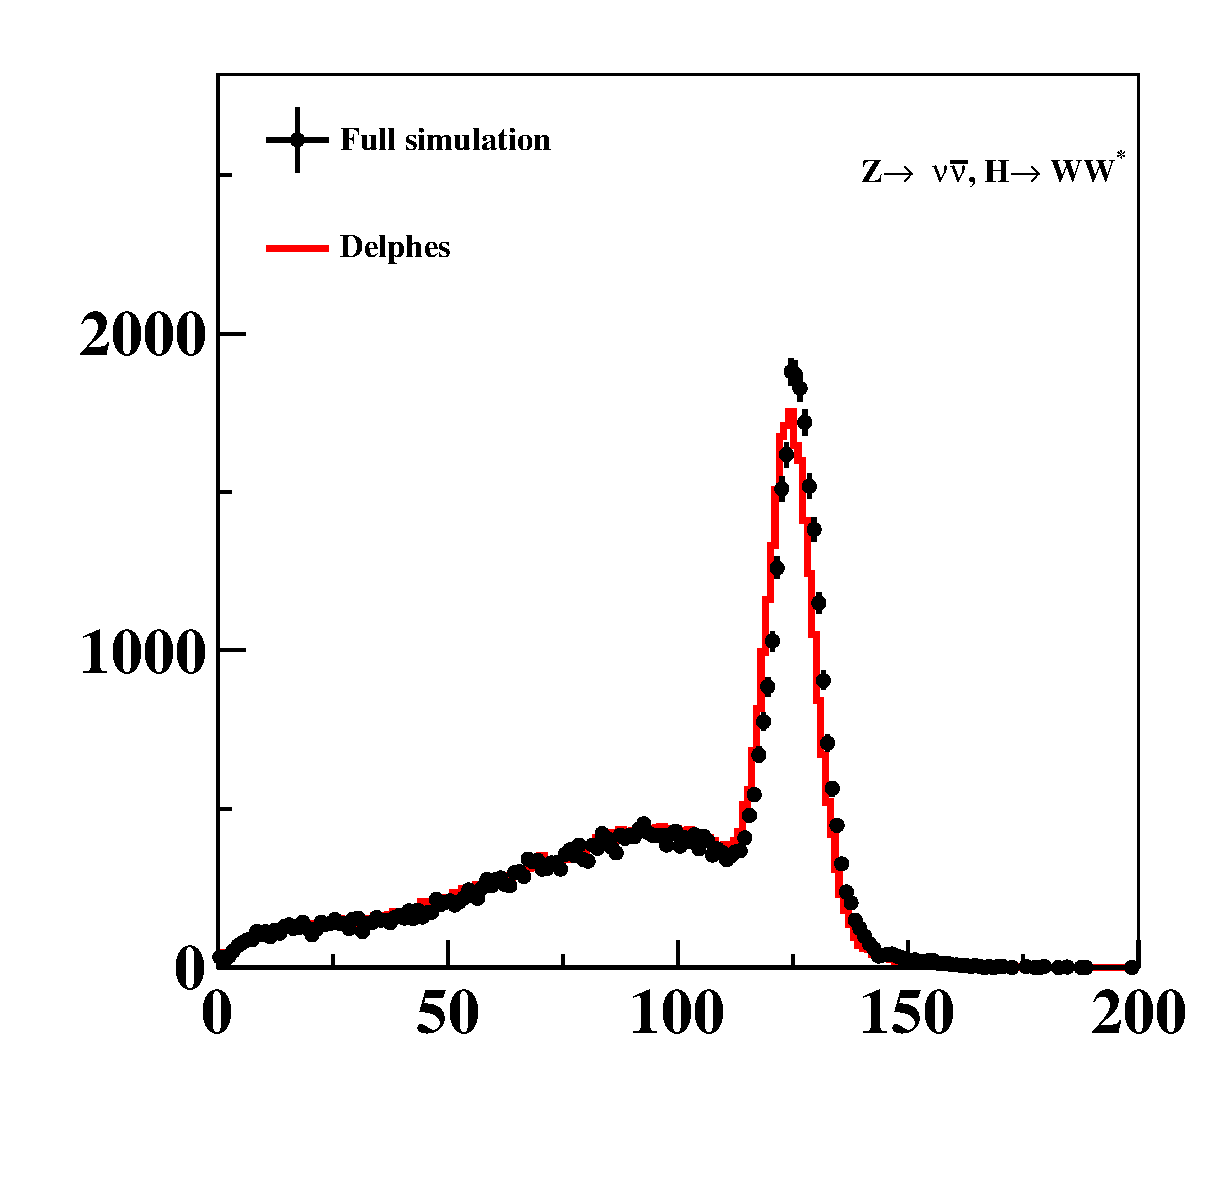
\includegraphics[width=0.4\linewidth]{figs/nnh_mass}
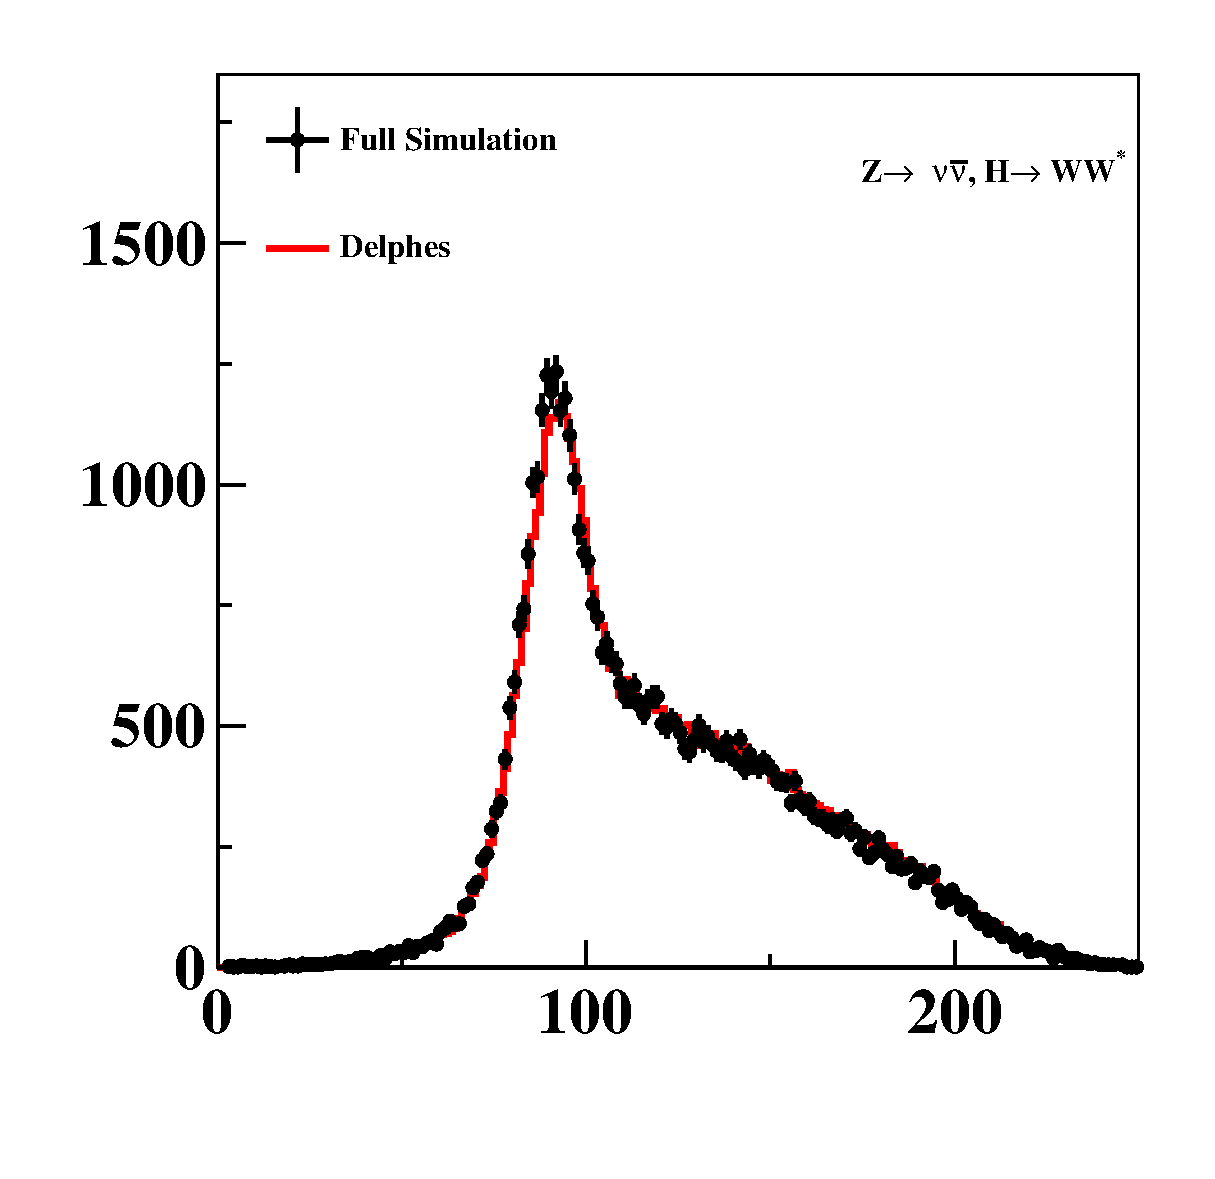
\includegraphics[width=0.4\linewidth]{figs/nnh_reco}
\figcaption{\label{fig:nnh} The distributions of invariant mass(left) of and recoil mass (right) against $WW^*$ system
  in $e^+e^- \to \nu\bar{\nu}H$, $H\to WW^{*}$.}
\end{center}

\subsection{$e^+e^- \to ZH \to 2(q\bar{q})$}

The $e^+e^- \to ZH \to 2(q\bar{q})$ process contains four jets in the final states, which is very useful
to validate the performances related jets, such as jet-clustering, jet energy resolution, and jet pairing, etc.
In both full and fast simulation, all the final states particles are forced into four jets with $ee_{kt}$ algorithm.
The four jets are paired by minimize $\chi^2 = (M_{j_1,j_2} - M_Z)^2 + (M_{j_3,j_4}-M_H)^2$,
where $M_Z$ and $M_H$ are the world averages of $Z$ and Higgs boson masses. 
The invariant mass distribution of jet pairs are shown in Fig.\ref{fig:zh4q}.
From Fig.~\ref{fig:zh4q}, it can be seen that both of the distributions are well consistent.
In Fig.~\ref{fig:zh4qsc}, the scattering plots of $M_{j_1,j_2}$  vs. $M_{j_3,j_4}$ 
demonstrate similar patterns in the available kinematic region.

\begin{center}
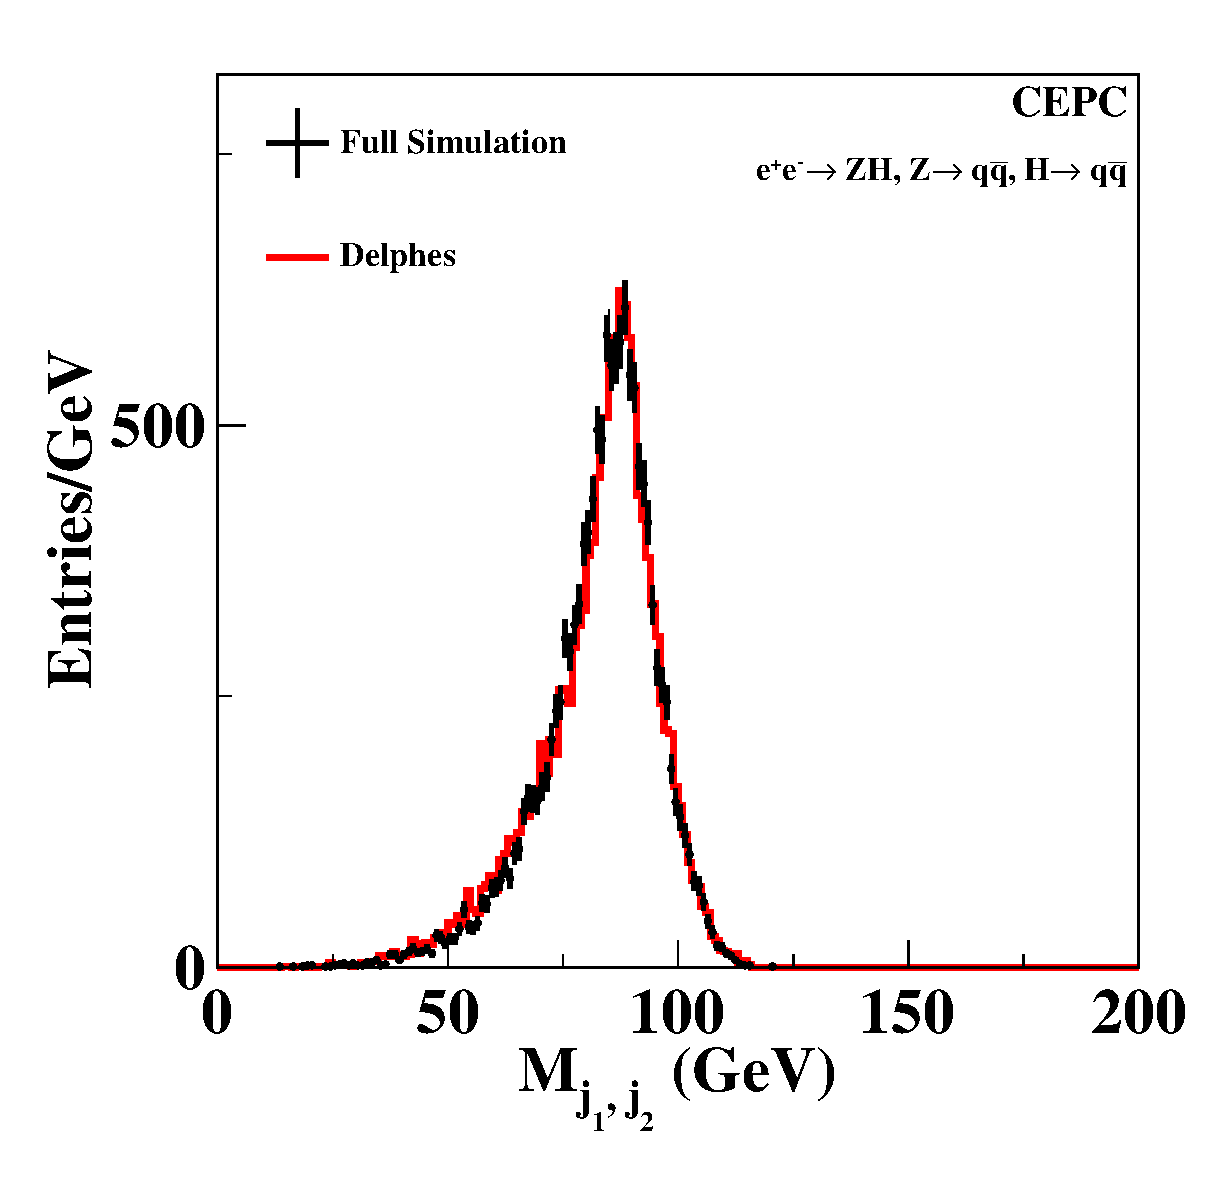
\includegraphics[width=0.45\linewidth]{figs/full_vs_delphes_z}
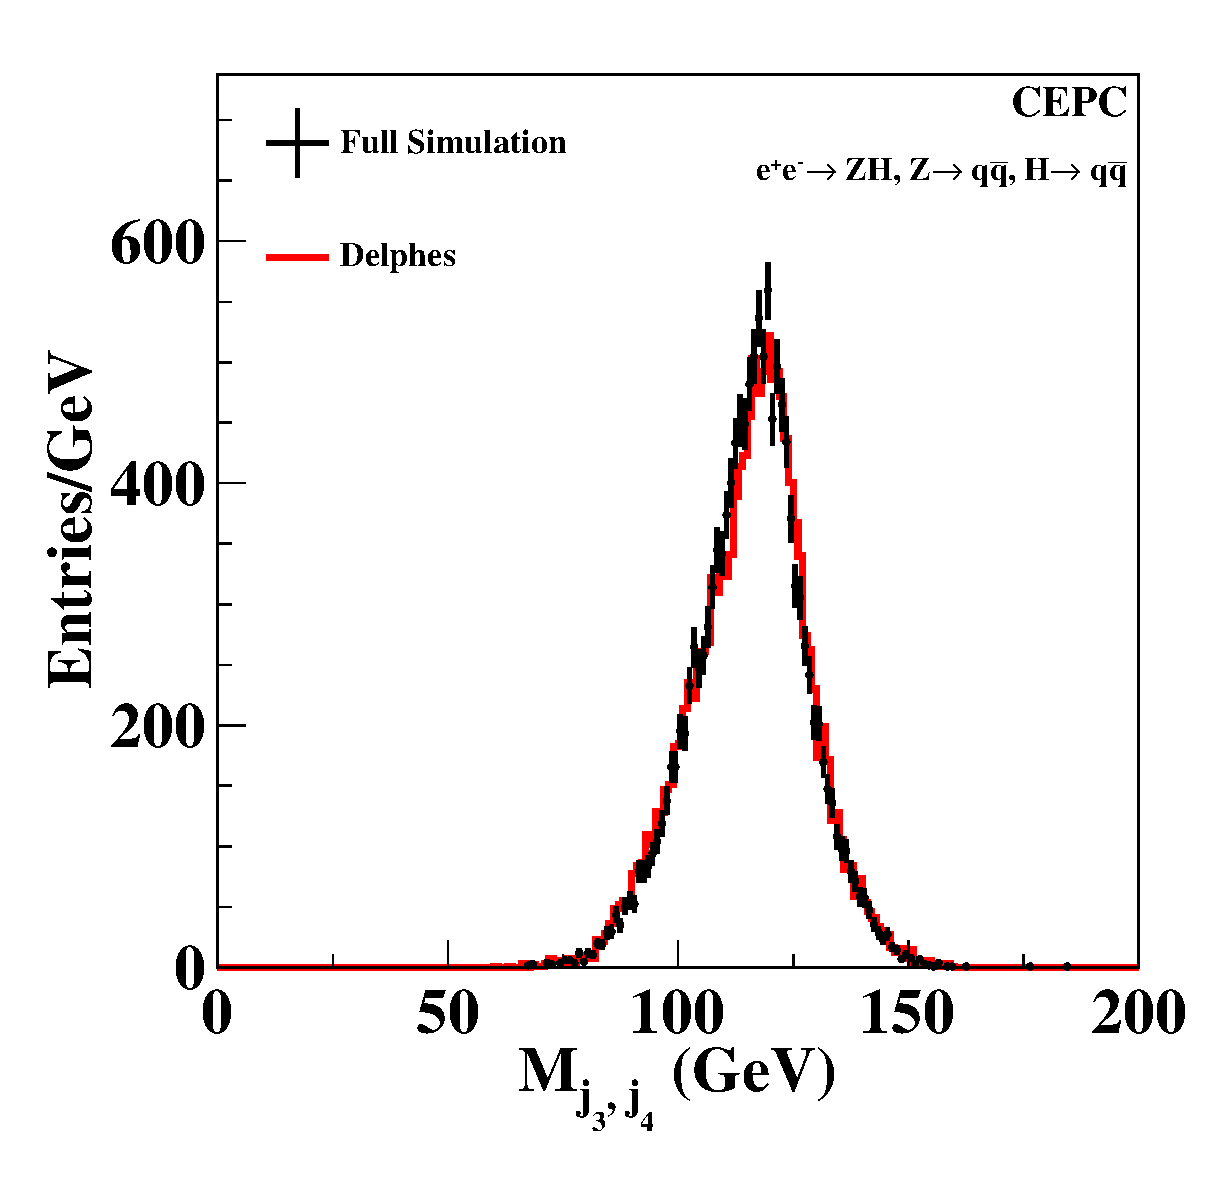
\includegraphics[width=0.45\linewidth]{figs/full_vs_delphes_h}
\figcaption{\label{fig:zh4q} The invariant mass distributions of the jet pairs, which are peaking at $Z$ and Higgs masses.}
\end{center}


\begin{center}
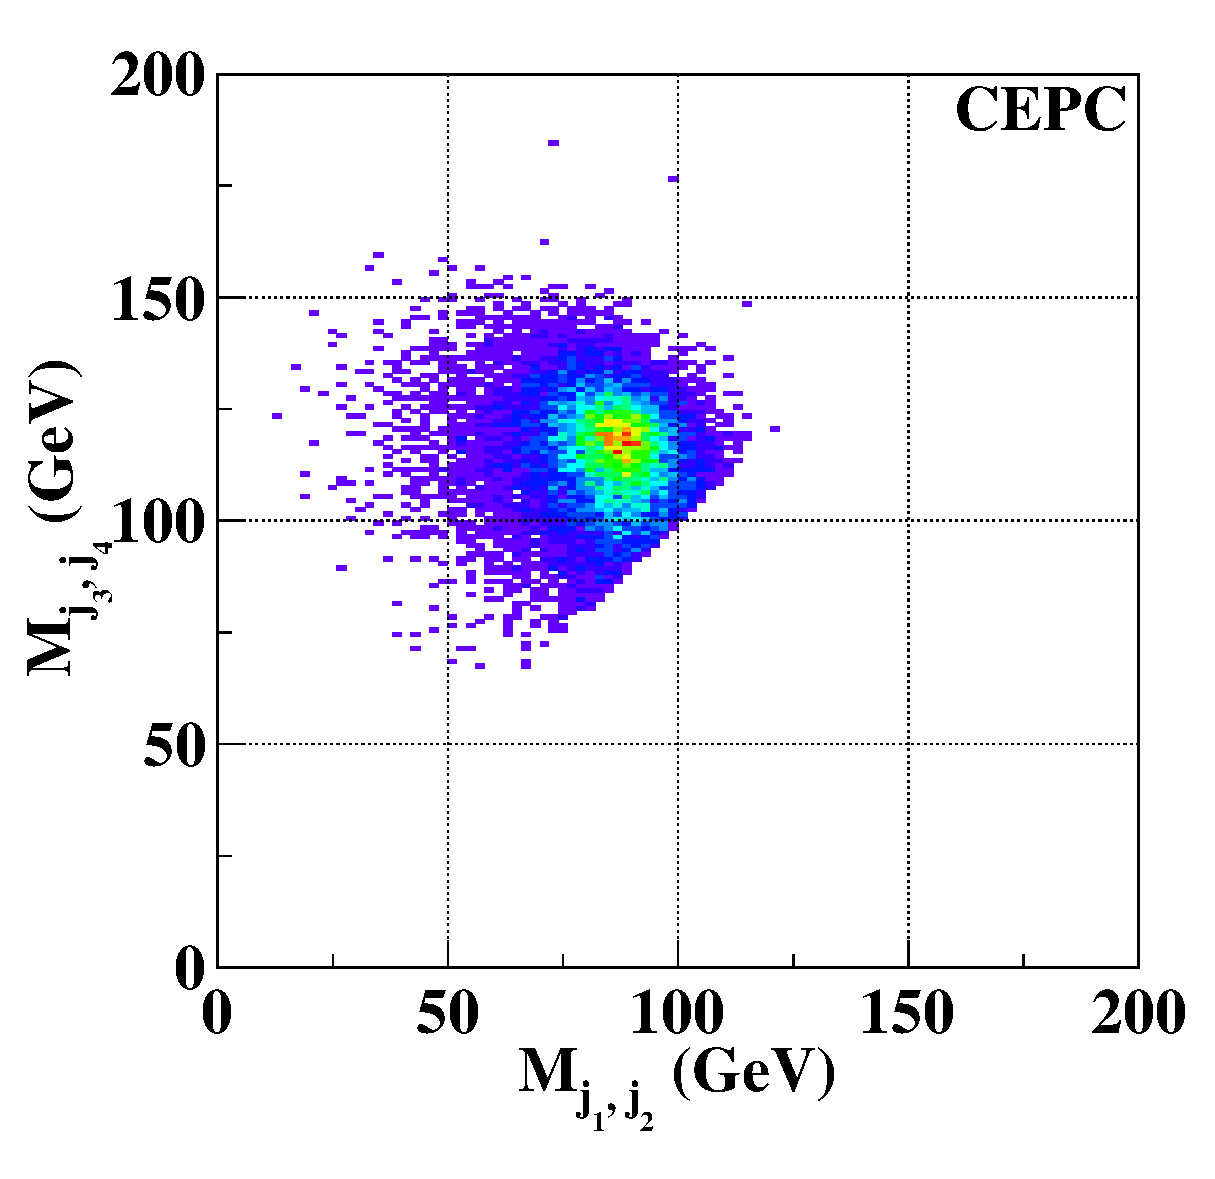
\includegraphics[width=0.48\linewidth]{figs/Full2DCOL}
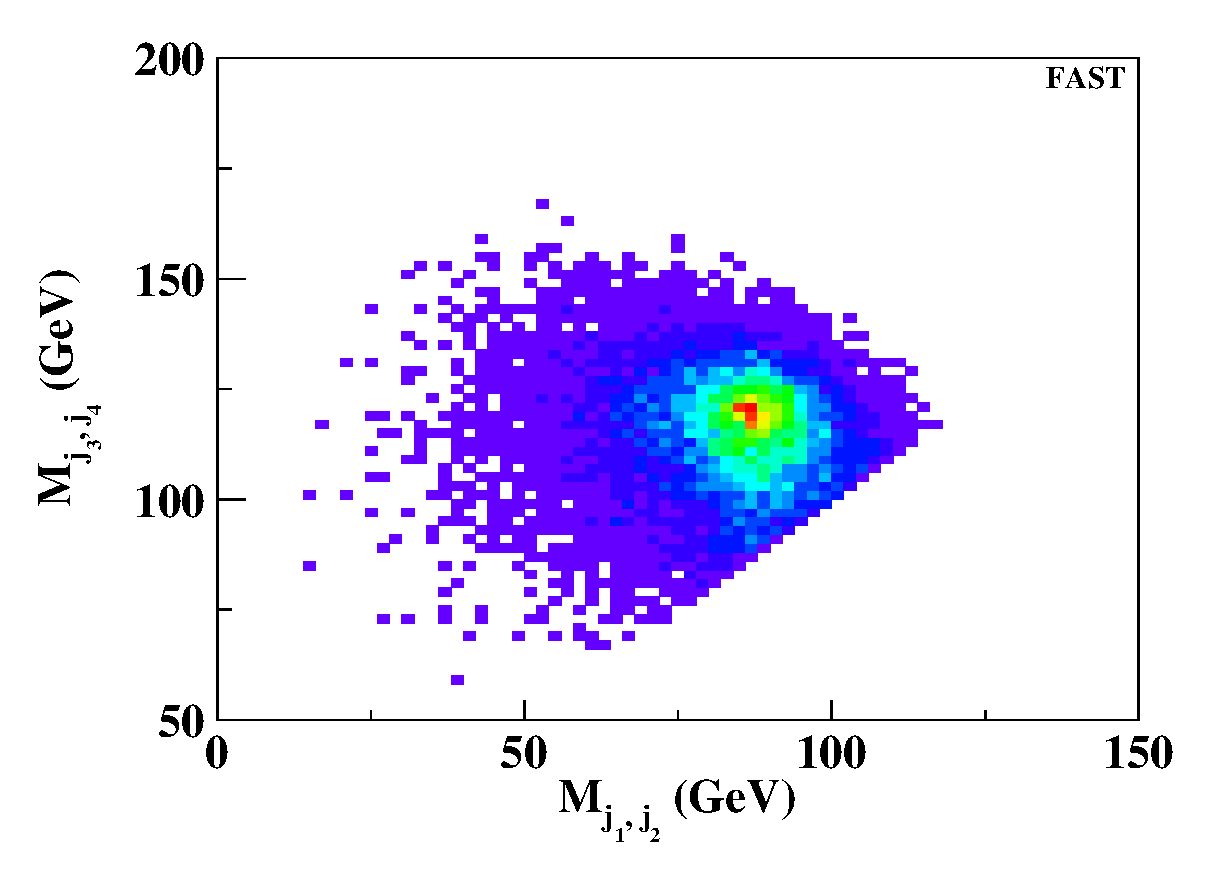
\includegraphics[width=0.48\linewidth]{figs/Fast2DCOL}
\figcaption{\label{fig:zh4qsc} The Scattering plots of $M_{j_1,j_2}$ vs. $M_{j_3,j_4}$ for full (the left) and fast (the right) simulations, respectively.}
\end{center}

\section{Flavor tagging based machine learning\label{b-tagging}}
In the original {\textsf{Delphes}}, the $b$-tagging is proceeding as following:
the jet becomes a potential $b$ jet candidate if a generated $b$ is found within
some distance $\Delta R = \sqrt{(\eta^{\mbox{\scriptsize jet}}-\eta^b)^2+(\phi^{\mbox{\scriptsize jet}}-\phi^b)^2}$ of the jet axis.
The probability to be identified as $b$ depends on user-defined parameterizations of the $b$ efficiency.
The user can also specify a mis-tagging efficiency parameterization.
But in the CEPC full simulation, the package LCFIPlus~\cite{ref:lcfiplus},
which is based on machine learning (BDT) approach, is used for $b/c$-tagging.
In this approach, jet flavor is identified based on a series of variables, up to 60, such as secondary vertex, jet shape and energy, etc.
LCFIPlus attaches two real numbers, $btag$ and $ctag$, to each jet,
which represent the probabilities of a jet to be a $b/c$ and light jet ($1-btag-ctag$).

In order to make a unified analysis procedure for fast and full simulations,
each jet in fast simulation is also attached the same two real numbers according to the flavor of the corresponding generated jet
and two dimensional distributions of $b/c$-likeliness of the full simulation.
\begin{center}
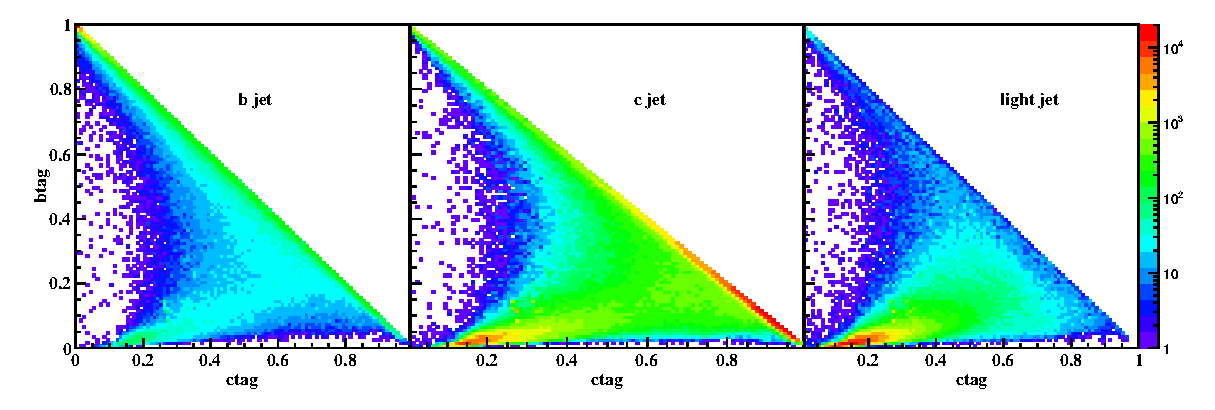
\includegraphics[width=0.95\linewidth]{figs/input}
\figcaption{\label{fig:input} Two dimensional distributions of $b$-likeliness versus $c$-likeliness for $b$, $c$ and light jets,
which are from full simulation and taken as input to fast simulation. }
\end{center}
\begin{center}
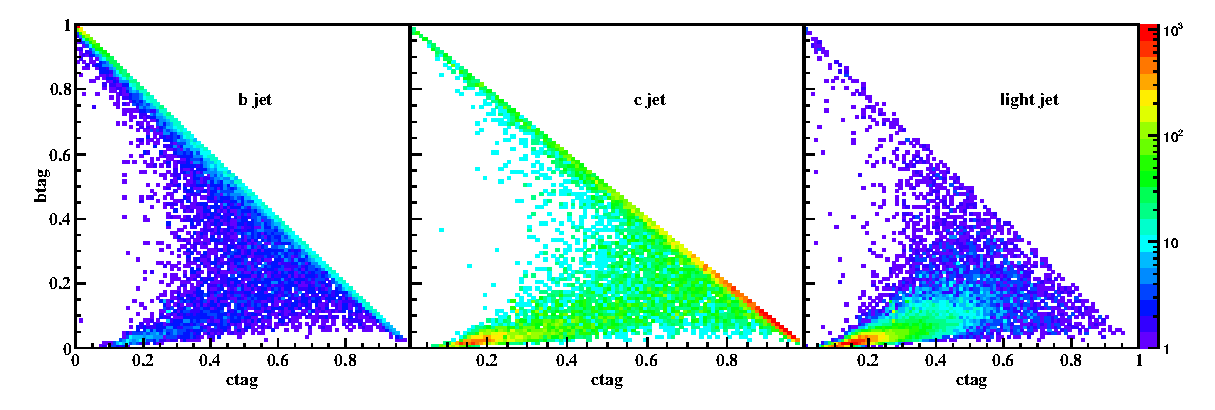
\includegraphics[width=0.95\linewidth]{figs/output}
\figcaption{\label{fig:output} Two dimensional distributions of $b$-likeliness versus $c$-likeliness for $b$, $c$ and light jets,
which are the output of fast simulation based on the full simulation input. }
\end{center}
Fig.~\ref{fig:input} and ~\ref{fig:output} demonstrate the input $b$-likeliness versus $c$-likeliness 
of various jet flavors of input distribution and the output fast simulation results, 
which can be seen that the fast simulation can reproduce the full simulation very well.
\section{Conclusion\label{sec:conclusion}}
A dedicated fast simulation tool is essential for the CEPC phenomenological study.
The fast simulation  frame work of the CEPC detector based {~\textsf{Delphes}~} is introduced. 
To validate the performance, comprehensive comparisons between {\textsc{Delphes}~} fast and full simulation are performed.
The results show  well agreement between fast and full simulations on the CEPC.

On the analyses in high energy $e^+e^-$ experiments, it worthy to note that exclusive jet-clustering algorithm is favored in most cases,
since it uses all final state particles and doesn't loose any available information. 
It also should be noted that the flavor tagging module are improved based on the machine learning results of full simulation, 
which is very useful since it provides a possibility to use the unified analysis procedure as full simulation.
\vspace{3mm}

\begin{thebibliography}{90}

\vspace{3mm}

\bibitem{ref:cepc_det}CEPC-SppC Preliminary Conceptual Design Report: Physics and Detector, by the CEPC Study Group.
\bibitem{ref:cepc_acc}CEPC Accelerator Preliminary Conceptual Design Report, by the CEPC Study Group.
\bibitem{ref:delphes}S. Ovyn, X. Rouby,  V. Lemaitre, {\textsc{Delphes}~}, a framework for fast simulation of a generic collider experiment, arXiv:0903.2225 [hep-ph].
\bibitem{ref:pfa}P. Janot, Particle Flow Event Reconstruction from LEP to LHC, Presented at Excellence in Detectors and Instrumentation Technologies workshop, CERN, 2011.
\bibitem{ref:ilc}T. Abe et al., The International Large Detector: Letter of Intent, arXiv:1006.3396 [hep-ex].
\bibitem{ref:ild}T. Behnke et al., The International Linear Collider Technical Design Report - Volume4:Detectors,arXiv:1306.6329 [physics.ins-det].
\bibitem{ref:cepccpc}X. Mo, G. Li, M. Ruan, X. Lou, Physics cross sections and event generation of $e^+e^-$ annihilations at the CEPC, Chi. Phys. C, 2016, {\bf 40}: 033001.
\bibitem{ref:whizard}W. Kilian, T. Ohl, J. Reuter, Eur. Phys. J. C, 2011, {\bf 71}:1742.
\bibitem{ref:mokka}  P.~Mora de Freitas and H.~Videau, LC-TOOL-2003-010.
\bibitem{ref:geant4}S. Agostinelli et al., GEANT4: A simulation toolkit, Nucl. Instrum. Meth. A, 2003, {\bf 506}:250.
\bibitem{ref:marlin} http://ilcsoft.desy.de/portal/software\_packages/marlin/index\_eng.html
\bibitem{ref:arbor}M. Ruan, H. Videau, Arbor, a new approach of the Particle Flow Algorithm, arXiv:1403.4784 [physics.ins-det]
\bibitem{ref:pandora}
  M.~A.~Thomson,
  Nucl.\ Instrum.\ Meth.\ A {\bf 611}, 25 (2009)
  doi:10.1016/j.nima.2009.09.009
  [arXiv:0907.3577 [physics.ins-det]].
\bibitem{ref:lcfiplus}
  T.~Suehara and T.~Tanabe,
  Nucl.\ Instrum.\ Meth.\ A {\bf 808}, 109 (2016)
  doi:10.1016/j.nima.2015.11.054
  [arXiv:1506.08371 [physics.ins-det]].
\bibitem{ref:eekt} S. Catani, Y. L. Dokshitzer, M. Olsson, G. Turnock and B. R. Webber, Phys. Lett. B {\bf 269}, 432 (1991);
%\bibitem{ref:antikt}M. Cacciari, G. P. Salam, G. Soyez, JHEP,2008, {\bf 04} :063 [arXiv:0802.1189 [hep-ph]].
\bibitem{ref:fastjet}M. Cacciari, G. P. Salam, Phys. Lett. B, 2006, {\bf 641}:57 [hep-ph/0512210], M. Cacciari, G.P. Salam, G. Soyez, Eur. Phys. J. C, 2012, {\bf 72}:1896[arXiv:1111.6097].
\bibitem{ref:lcio}F. Gaede, T. Behnke, N. Graf, T. Johnson, arXiv:physics/0306114.

\end{thebibliography}
\end{multicols}

\clearpage

\end{document}
